\documentclass[tikz, border=10pt]{standalone}
\usepackage{pgfplots}
\usepackage[american]{circuitikz}
\usepgfplotslibrary{groupplots}
\pgfplotsset{compat=1.18}

\begin{document}
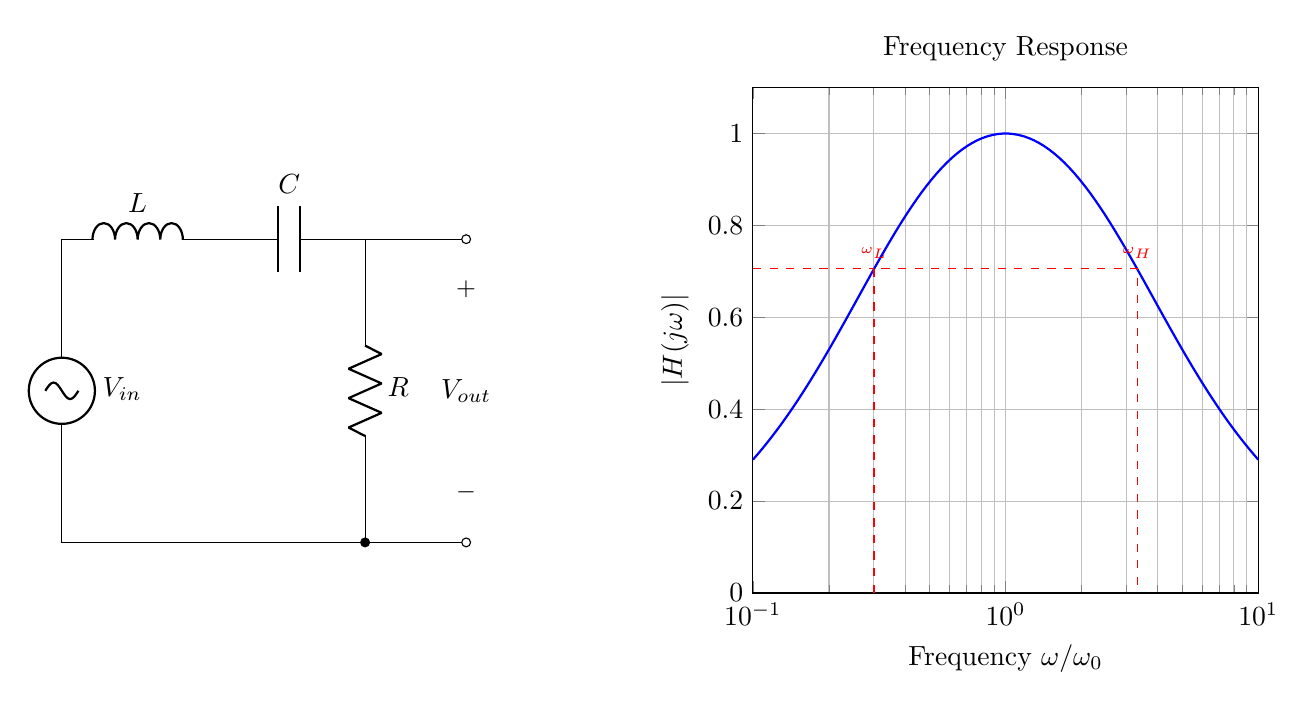
\begin{tikzpicture}
    \begin{groupplot}[
        group style={
            group size=2 by 1,
            horizontal sep=3cm,
        },
        width=8cm, height=8cm,
    ]
    
    % Schematic
    \nextgroupplot[
        axis lines=none,
        xmin=0, xmax=1,
        ymin=0, ymax=1,
    ]
    \draw (axis cs: 0.1, 0.7) to [sV, l=$V_{in}$] (axis cs: 0.1, 0.1)
          to [short] (axis cs: 0.9, 0.1);
    \draw (axis cs: 0.1, 0.7) to [L, l=$L$] (axis cs: 0.4, 0.7)
          to [C, l=$C$] (axis cs: 0.7, 0.7)
          to [R, l=$R$, -*] (axis cs: 0.7, 0.1);
    \draw (axis cs: 0.7, 0.7) to [short, -o] (axis cs: 0.9, 0.7);
    \draw (axis cs: 0.7, 0.1) to [short, -o] (axis cs: 0.9, 0.1);
    
    \node at (axis cs: 0.9, 0.6) {\small $+$};
    \node at (axis cs: 0.9, 0.4) {$V_{out}$};
    \node at (axis cs: 0.9, 0.2) {\small $-$};
    
    % Response Plot
    \nextgroupplot[
        title={Frequency Response},
        xlabel={Frequency $\omega/\omega_0$},
        ylabel={$|H(j\omega)|$},
        xmin=0.1, xmax=10,
        xmode=log,
        ymin=0, ymax=1.1,
        grid=both,
    ]
    % H(s) = (sR/L) / (s^2 + sR/L + 1/LC)
    % Let zeta = 1/(2Q)
    % |H| = (omega*R/L) / sqrt( (1/LC - omega^2)^2 + (omega*R/L)^2 )
    % In terms of omega/omega0:
    % |H| = ( (omega/omega0) * (1/Q) ) / sqrt( (1 - (omega/omega0)^2)^2 + ( (omega/omega0)/Q )^2 )
    % Let Q = 1/3 (wide band as in example)
    \addplot[thick, blue, variable=\t, domain=-1:1, samples=100] ({10^\t}, { ( (10^\t) * 3 ) / sqrt( (1 - (10^\t)^2)^2 + ((10^\t)*3)^2 ) });
    
    % Mark Cutoffs
    % For Q=1/3, cutoffs are at 1/omega0 and 10/omega0? No.
    % f1 = 0.1 MHz, f2 = 1.1 MHz, f0 = 0.33 MHz. 
    % omega1/omega0 = 0.1/0.33 = 0.3
    % omega2/omega0 = 1.1/0.33 = 3.3
    \draw[dashed, red] (axis cs: 0.3015, 0) -- (axis cs: 0.3015, 0.707) -- (axis cs: 3.316, 0.707) -- (axis cs: 3.316, 0);
    \draw[dashed, red] (axis cs: 0.1, 0.707) -- (axis cs: 0.3015, 0.707);
    
    \node[anchor=south, red, font=\tiny] at (axis cs: 0.3015, 0.707) {$\omega_L$};
    \node[anchor=south, red, font=\tiny] at (axis cs: 3.316, 0.707) {$\omega_H$};

    \end{groupplot}
\end{tikzpicture}
\end{document}
